% !TeX program = xelatex
\documentclass[10pt,a4paper]{ctexart} % 设置文章类型，正文字号与纸张大小

% 页面与正文常用宏包
\usepackage[margin=2cm]{geometry} % 设置页面四周页边距
\usepackage{graphicx}             % 插入图片
\usepackage{amsmath}              % 提供cases、aligned等数学公式环境
\usepackage{amssymb}              % 提供\therefore等扩展数学符号
\usepackage{booktabs}             % 提供\toprule、\midrule、\bottomrule三线表命令
\usepackage{float}                % 提供[H]固定图片、表格位置
\usepackage{subcaption}           % 提供subfigure子图环境及子图标题
\usepackage{wrapfig}              % 提供wrapfigure图文环绕环境
\usepackage{fancyhdr}             % 自定义页眉和页脚
\usepackage{hyperref}             % 生成超链接

% 页眉页脚
\pagestyle{fancy}                  % 启用fancyhdr定义的页面样式
\fancyhf{}                         % 清空默认页眉和页脚
\fancyfoot[C]{\thepage}            % 在页脚中央显示页码
\renewcommand{\headrulewidth}{0pt} % 隐藏页眉横线
\renewcommand{\footrulewidth}{0pt} % 隐藏页脚横线

% 超链接
\hypersetup{
  colorlinks=true,                % 使用彩色文字链接，而非带边框的链接
  linkcolor=red,                 % 目录、公式及图表交叉引用的颜色
  filecolor=cyan,                 % 本地文件链接的颜色
  urlcolor=blue,                  % 网址链接的颜色
  pdftitle={双棱镜干涉预习报告},     % 写入PDF文档属性的标题
  bookmarksnumbered=true          % PDF书签显示章节编号
}

% 定义字号命令
\newcommand{\chuhao}{\fontsize{42pt}{63pt}\selectfont}
\newcommand{\xiaochu}{\fontsize{36pt}{54pt}\selectfont}
\newcommand{\yihao}{\fontsize{26pt}{39pt}\selectfont}
\newcommand{\xiaoyi}{\fontsize{24pt}{36pt}\selectfont}
\newcommand{\erhao}{\fontsize{22pt}{33pt}\selectfont}
\newcommand{\xiaoer}{\fontsize{18pt}{27pt}\selectfont}
\newcommand{\sanhao}{\fontsize{16pt}{24pt}\selectfont}
\newcommand{\xiaosan}{\fontsize{15pt}{22.5pt}\selectfont}
\newcommand{\sihao}{\fontsize{14pt}{21pt}\selectfont}
\newcommand{\xiaosi}{\fontsize{12pt}{18pt}\selectfont}
\newcommand{\wuhao}{\fontsize{10.5pt}{15.75pt}\selectfont}
\newcommand{\xiaowu}{\fontsize{9pt}{13.5pt}\selectfont}

% 章节格式
\ctexset{
  section={
    format={\CJKfontspec[AutoFakeBold=2.5]{KaiTi}\sanhao\bfseries}, % 一级标题使用三号加粗楷体
    beforeskip=1.5ex, afterskip=1ex,
    name={,、},                                                    % 在中文章节序号后添加顿号
    number=\chinese{section},                                      % 一级标题编号使用“一、二、三”形式
    aftername={}                                                   % 取消编号与标题文字之间的空格
  },
  subsection={
    beforeskip=1.5ex, afterskip=0.8ex,
    format={\CJKfontspec[AutoFakeBold=2.5]{KaiTi}\sihao\bfseries}, % 二级标题使用四号加粗楷体
  },
  subsubsection={
    beforeskip=1.2ex, afterskip=0.6ex,
    format={\CJKfontspec[AutoFakeBold=2.5]{KaiTi}\xiaosi\bfseries}, % 三级标题使用小四加粗楷体
  }
}

\begin{document}

% 封面
\thispagestyle{fancy} % 封面保留底部居中的页码
\fancyfoot[C]{\thepage}
\begin{center}
  \CJKfontspec[AutoFakeBold=2.5]{KaiTi}\bfseries % 封面中文使用楷体并人工加粗，西文同时加粗
  \vspace*{2.0cm}
  \xiaochu 
    物理实验预习报告

  \vspace{3.8cm}
  \begin{minipage}{10.0cm}
    \sanhao
    \makebox[2.6cm][l]{实验名称：}
    \underline{\makebox[7.0cm][c]{双棱镜干涉}}\par\vspace{12pt}

    \makebox[2.6cm][l]{指导老师：}
    \underline{\makebox[7.0cm][c]{包泽杭}}\par\vspace{12pt}
  \end{minipage}

  \vspace{3.8cm}
  \begin{minipage}{10.0cm}
    \sihao
    \makebox[1.4cm][l]{班级：}
    \underline{\makebox[8.0cm][c]{}}\par\vspace{10pt}

    \makebox[1.4cm][l]{姓名：}
    \underline{\makebox[8.0cm][c]{IllusoryRain}}\par\vspace{10pt}

    \makebox[1.4cm][l]{学号：}
    \underline{\makebox[8.0cm][c]{}}
  \end{minipage}

  \vspace{1.8cm}
  \sihao
    实验日期：
    \underline{\makebox[0.7cm][c]{2026}}年
    \underline{\makebox[0.7cm][c]{11}}月
    \underline{\makebox[0.7cm][c]{4}}日
    星期\underline{\makebox[0.7cm][c]{三}}上午

  \vspace{0.7cm}
  \sihao 
    浙江大学物理实验教学中心
\end{center}

\newpage
\xiaosi\songti\mdseries % 后续正文统一使用小四不加粗的宋体

\section{预习报告（10分）}

  \subsection{实验综述（5分）}
  
    \subsubsection{凸透镜成像原理}
    凸透镜满足成像公式
    \[
    \frac{1}{f}=\frac{1}{u}+\frac{1}{v},\qquad u+v=D
    \]
    
    其中，\(u\)、\(v\)分别为物距和像距，\(D\)为物屏间距。当\(D>4f\)时，移动透镜可在屏上先后得到放大像和缩小像，
    两次成像的物距与像距互换。若两次透镜位置相距\(\Delta l\)，则
    \[
    f=\frac{D^2-\Delta l^2}{4D}
    \]
    
    当\(D=4f\)时，两个成像位置重合。

    \subsubsection{光的干涉原理}
    两束光频率相同、振动方向一致且相位差恒定时，可产生稳定的干涉条纹。
    相干光可通过分波前法（如杨氏双缝、菲涅尔双棱镜）或分振幅法（如薄膜干涉、迈克尔逊干涉仪）获得。

    对于初相位相同的两束相干光，明暗条纹的光程差条件为
    \[
    \delta=
    \begin{cases}
      k\lambda, & \text{明纹},\\[4pt]
      (k+\frac{1}{2})\lambda, & \text{暗纹},
    \end{cases}
    \qquad k\in\mathbb{Z}
    \]

    \begin{figure}[H]
      \centering
      \begin{minipage}{0.33\textwidth}
        \centering
        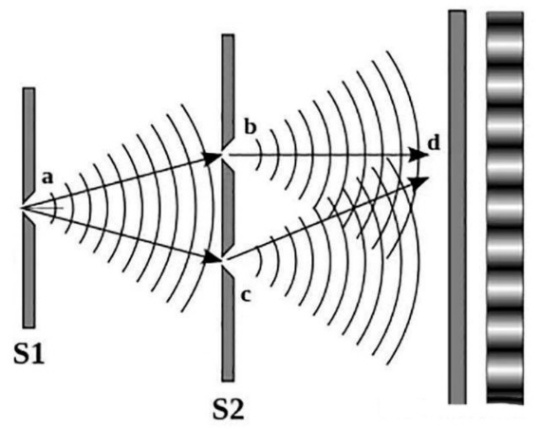
\includegraphics[width=\linewidth]{figures/图1.png}
        \caption{分波前法}
      \end{minipage}
      \hfill
      \begin{minipage}{0.33\textwidth}
        \centering
        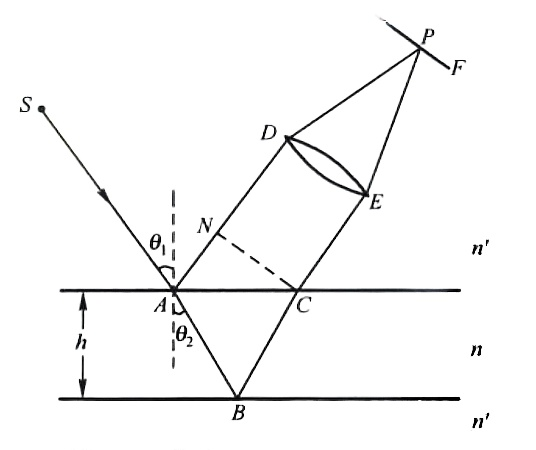
\includegraphics[width=\linewidth]{figures/图2.png}
        \caption{分振幅法}
      \end{minipage}
    \end{figure}

    \subsubsection{波长测量原理}
    双棱镜将同一狭缝发出的光分成两束，相当于两个相干虚光源。设虚光源间距为\(d\)，虚光源到观察屏的距离为\(D\)，
    屏上某点距条纹中心为\(x\)，在小角度近似下，光程差为
    \[
    \delta\approx\frac{dx}{D}
    \]
    
    相邻暗纹的光程差相差一个波长，因此条纹间距\(\Delta x\)满足
    \[
    \lambda=\frac{d\,\Delta x}{D}
    \]
    
    虚光源的位置和间距难以直接测量，实验中利用凸透镜二次成像法求得\(d\)和\(D\)，再测量\(\Delta x\)计算波长。

    \subsubsection{实验内容}
    \begin{enumerate}
      \item 光路调节：调节各元件等高共轴，依次调整透镜、狭缝、双棱镜和摄像头，使像与叉丝清晰可辨。
      \item 二次成像测量：在双棱镜与毛玻璃屏之间沿光轴移动透镜，找到分别形成放大像、缩小像的两个清晰位置，记录透镜位置及对应的像点间距，求出\(d\)和\(D\)。测量时，移动摄像头，使叉丝竖线对准像点中心；若像点过亮，可适当调小狭缝。
      \item 条纹间距测量：移开透镜，微调狭缝宽度，使干涉条纹与叉丝均清晰可辨。转动摄像头底座的螺旋测微器，对暗纹两侧明暗交界线分别读数，取平均值作为暗纹中心位置，据此求得条纹间距并计算波长。
    \end{enumerate}

  \subsection{实验重点（3分）}
  \begin{enumerate}
    \item 掌握分波面法干涉原理。
    \item 了解双棱镜干涉装置及光路调节技巧。
    \item 观察双棱镜干涉现象并测定光波波长。
  \end{enumerate}

  \subsection{实验难点（2分）}
  \begin{enumerate}
    \item 完成等高共轴调节，并通过狭缝宽度调节获得清晰条纹。
    \item 准确找到两个清晰成像位置，测量像点间距及相关距离。
    \item 准确定位暗纹中心，减小读数误差。
  \end{enumerate}

\vspace*{\fill} % 使下面内容在页面底部显示
\noindent
\begin{minipage}{\textwidth}
  注意事项：

  \begingroup
    \setlength{\leftskip}{2em} % 1--4整体向右缩进两个汉字宽度
    1. 用PDF格式上传“实验报告”，文件名：学生姓名+学号+实验名称+周次。

    2. “实验报告”必须递交在“学在浙大”本课程内对应实验项目的“作业”模块内。

    3. “实验报告”成绩必须在“浙江大学物理实验教学中心网站”-“选课系统”内查询。

    4. 教学评价必须在“浙江大学物理实验教学中心网站”-“选课系统”内进行，学生必须进行教学评价，才能看到实验报告成绩，教学评价须在本次实验结束之后3天内进行。\par
  \endgroup

  \begin{center}
    {\CJKfontspec[AutoFakeBold=2.5]{SimSun}\bfseries 浙江大学物理实验教学中心制}
  \end{center}
\end{minipage}

\end{document}

